\subsection{Amministratore}
\subsubsection{Panoramica Amministratore}
DA FARE


\subsubsection{UC5.1 - Visualizzazione elenco utenti}

\begin{figure}[H]
\centering
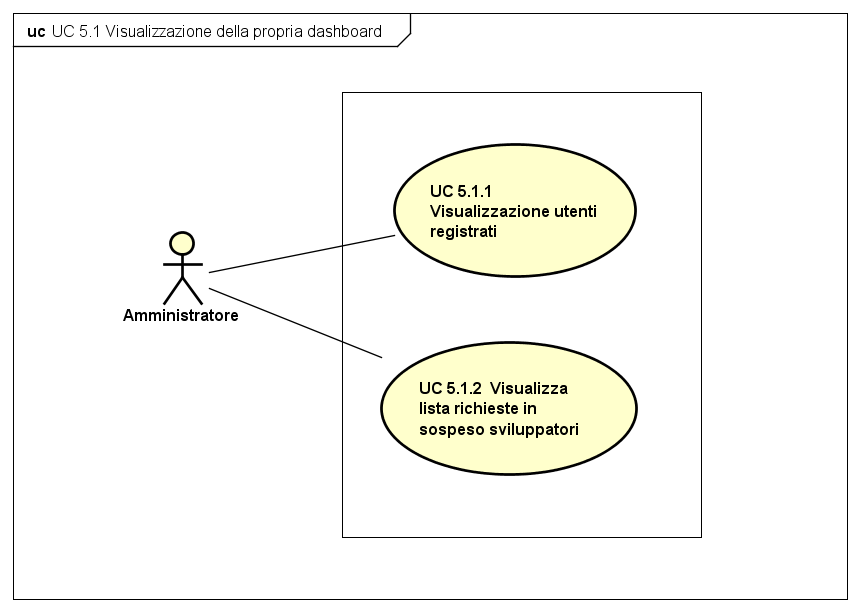
\includegraphics[width=17cm]{img/UC51.png} 
\caption{Caso d'uso UC5.1}
\end{figure}


\begin{itemize}
\item[•] \textbf{Attore}: Amministratore;

\item[•] \textbf{Descrizione}: L'amministratore visualizza l'elenco degli utenti nel sistema che sono registrati;

\item[•] \textbf{Precondizione}: L'amministratore si è autenticato nel sistema e visualizza la propria dashboard;

\item[•] \textbf{Postcondizione}: L'amministratore visualizza l'elenco degli utenti presenti nel sistema;

\item[•] \textbf{Flusso degli eventi}: L'amministratore accede alla pagina contenete l'elenco degli utenti e visualizza i dati degli utenti. 


\subsubsection{UC5.2 - Visualizzazione elenco richieste}

\begin{figure}[H]
\centering
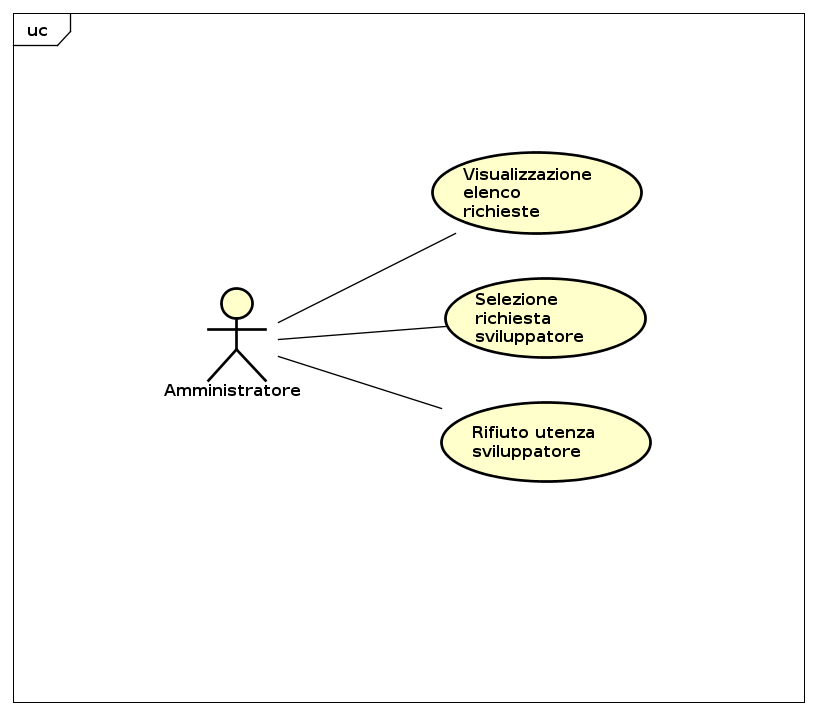
\includegraphics[width=17cm]{img/UC52.png} 
\caption{Caso d'uso UC5.2}
\end{figure}


\begin{itemize}
\item[•] \textbf{Attore}: Amministratore;

\item[•] \textbf{Descrizione}: L'amministratore visualizza l'elenco delle richieste provenienti da utenti che intendono registrarsi nel sistema come sviluppatori;

\item[•] \textbf{Precondizione}: L'amministratore si è autenticato nel sistema e visualizza la propria dashboard;

\item[•] \textbf{Postcondizione}: L'amministratore visualizza l'elenco delle richieste effettuate che devono ancora essere gestite;

\item[•] \textbf{Flusso degli eventi}: L'amministratore accede alla pagina contenete l'elenco delle richieste che necessitano di un intervento da parte dell'amministratore.

\subsubsection{UC5.3 - Approvazione registrazione}
\begin{figure}[H]
\centering
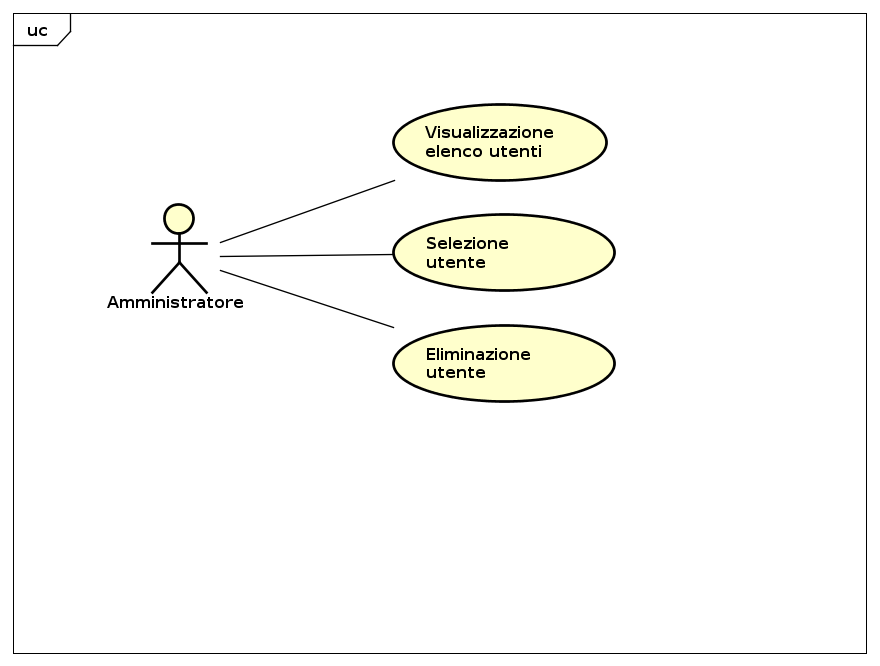
\includegraphics[width=17cm, height=9cm]{img/UC53.png} 
\caption{Caso d'uso UC5.3}
\end{figure}

\begin{itemize}
\item[•] \textbf{Attore}: Amministratore;

\item[•] \textbf{Descrizione}: L'amministratore approva la richiesta di registrazione da parte dello sviluppatore;

\item[•] \textbf{Precondizione}: Lo sviluppatore ha effettuato richiesta di registrazione, l'amministratore visualizza le richieste di registrazione da parte degli sviluppatori che desiderano accedere ai dati della piattaforma;

\item[•] \textbf{Postcondizione}: L'amministratore approva la richiesta di registrazione sviluppatore che quindi può registrarsi;

\item[•] \textbf{Flusso degli eventi}:

\begin{enumerate}

\item UC 5.2 - Visualizzazione elenco richieste;

\item Selezione richiesta sviluppatore;

\item Approvazione richiesta sviluppatore.

\end{enumerate}

\end{itemize}


\subsubsection{UC5.4 - Rifiuto registrazione}

\begin{figure}[H]
\centering
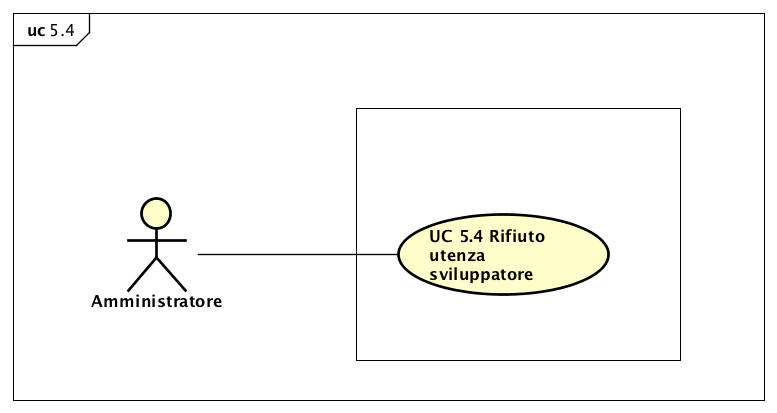
\includegraphics[width=11cm]{img/UC54.png} 
\caption{Caso d'uso UC5.4}
\end{figure}


\begin{itemize}
\item[•] \textbf{Attore}: Amministratore;

\item[•] \textbf{Descrizione}: L’amministratore rifiuta la richiesta di registrazione da parte dello sviluppatore;

\item[•] \textbf{Precondizione}: Lo sviluppatore ha richiesto l'approvazione, l'amministratore visualizza la richiesta di registrazione da parte dello sviluppatore che desidera accedere ai dati della piattaforma;

\item[•] \textbf{Postcondizione}: L'amministratore rifiuta la richiesta di registrazione dello sviluppatore;

\item[•] \textbf{Flusso degli eventi}:

\begin{enumerate}

\item UC 5.2 - Visualizzazione elenco richieste;

\item Selezione richiesta sviluppatore;

\item Rifiuto utenza sviluppatore.

\end{enumerate}
\end{itemize}
\subsubsection{UC5.5- Eliminazione utenza}
\begin{figure}[H]
\centering
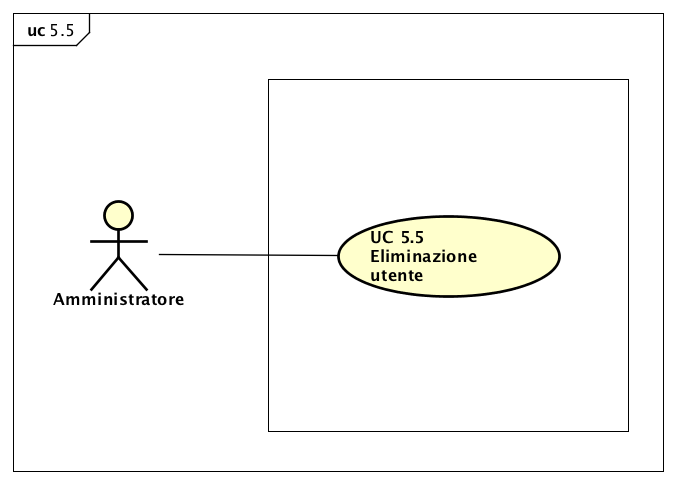
\includegraphics[width=11cm]{img/UC55.png} 
\caption{Caso d'uso UC5.5}
\end{figure}
\begin{itemize}
\item[•] \textbf{Attore}: Amministratore;

\item[•] \textbf{Descrizione}: L’amministratore elimina un’utenza dal sistema;

\item[•] \textbf{Precondizione}: L’amministratore \`{e} autenticato e visualizza l’elenco degli utenti nel sistema, e l’utenza da eliminare \`{e} registrata nel sistema;

\item[•] \textbf{Postcondizione}: L'amministratore ha eliminato l'utenza dal sistema; 

\item[•] \textbf{Flusso degli eventi}:

\begin{enumerate}

\item UC 5.1 - Visualizzazione elenco utenti;

\item Selezione utente;

\item Eliminazione utente.

\end{enumerate}

\end{itemize}
